\documentclass[11pt,a4paper]{article}
\usepackage[T1]{fontenc}
\usepackage[margin=2.3cm]{geometry}
\usepackage{amsmath,amssymb}
\usepackage{graphicx}
\usepackage[dvipsnames]{xcolor}
\usepackage{enumitem}
\usepackage[colorlinks=true,linkcolor=blue,urlcolor=blue]{hyperref}
\setlength{\parskip}{0.6em}
\setlength{\parindent}{0pt}
\begin{document}

\begin{center}{\LARGE\bfseries openrobotarm}\\[0.4em]{\large Make a robot arm pick and place: from joint angles to the gripper and back, in three sessions.}\\[0.2em]\small PAN IIT OSS explainer \textbullet{} higher secondary to advanced undergraduate (levels 4-6)\end{center}

\section*{Why this exists}
A robot arm is a chain of rigid links joined by motors. This explainer shows the mathematics that links the angles of the motors to the position of the gripper, and back, using only sines, cosines and small matrices, so you can build it yourself.

\section*{The end goal}
Forward and inverse kinematics for a pick-and-place arm. The end goal is forward and inverse kinematics for a pick-and-place arm: find where the gripper is from the joint angles, and find joint angles that put it where we want, along a smooth path, within the limits of the machine. The same mathematics drives character rigs in film and the mechanisms of machines.

\section*{How the three sessions build up}
\begin{enumerate}[nosep]
\item \textbf{Session 1: A robot arm is a chain of links and joints} (Level 1, conceptual interactive model, 60 min).
\item \textbf{Session 2: Where can the gripper go? Workspace, joint limits and redundancy} (Level 2, mathematical engineering model, 80 min).
\item \textbf{Session 3: Numerical inverse kinematics and a pick-and-place path} (Level 3, simulation and validation, 90 min).
\end{enumerate}

\section{Session 1: A robot arm is a chain of links and joints}

\subsection*{A. Real-world problem}
A pick-and-place robot lifts a block from one spot and sets it down on another, hundreds of times an hour. Its motors only turn joints. Nobody can tell a motor 'go to x = 0.40, y = 0.30'; we must work out which joint angles put the gripper there. Before running the problem backwards, we must be able to run it forwards: given three joint angles, where does the gripper end up? Can a 3-link arm with links of 0.30 m, 0.25 m and 0.15 m touch a block 0.40 m across and 0.30 m up?

\subsection*{B. Concept and theory}
The arm is a chain: link 1 is fixed to the base at the origin by joint 1, link 2 is fixed to the end of link 1 by joint 2, and so on. Each joint angle is measured relative to the previous link, so a link's direction in the room is the running total of the joint angles up to it (its cumulative angle). Walking along the chain, each link adds its length times (cos, sin) of its cumulative angle, and the last point is the gripper. The tool angle, the direction the gripper points, is the sum of all joint angles. The gripper can never be farther from the base than the sum of the link lengths.

\begin{itemize}[nosep]
\item q1, q2, q3: joint angles, each relative to the previous link, counter-clockwise positive (degrees or radians)
\item L1, L2, L3: link lengths (0.30, 0.25, 0.15) (m)
\item c1, c2, c3: cumulative angles: direction of each link from the x axis (degrees or radians)
\item (x, y): gripper position (m)
\item tool angle: direction the gripper points, q1 + q2 + q3 (degrees)
\end{itemize}

\begin{equation*}
c_k=q_1+q_2+\cdots+q_k
\end{equation*}

\begin{equation*}
x=\sum_{k=1}^{3}L_k\cos c_k,\qquad y=\sum_{k=1}^{3}L_k\sin c_k
\end{equation*}

\begin{equation*}
\text{tool angle}=c_3=q_1+q_2+q_3
\end{equation*}

\begin{equation*}
\sqrt{x^2+y^2}\le L_1+L_2+L_3=0.70\ \text{m}
\end{equation*}

\begin{center}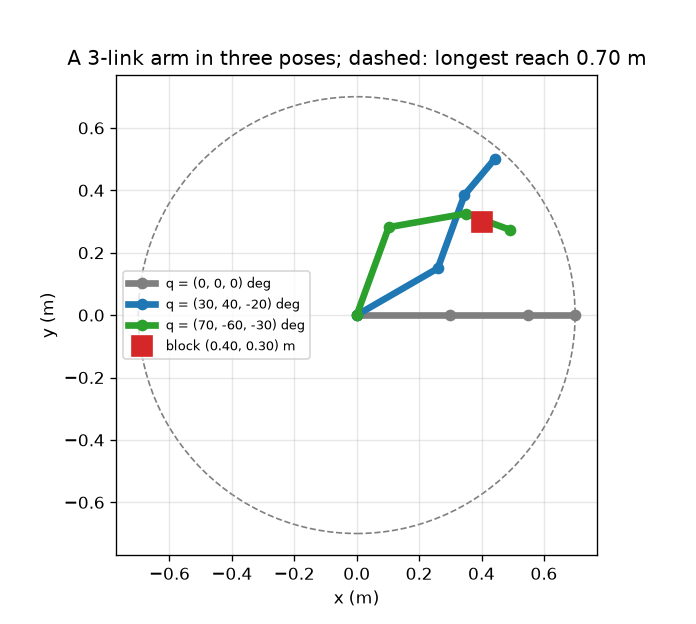
\includegraphics[width=0.85\linewidth]{figures/s01_arm_poses.png}\\\small Three poses of the 3-link arm in metres, the block and the longest reach.\end{center}

\subsection*{E. Worked example}
Find the gripper position, the tool angle and the distance from the base for q = (30, 40, -20) degrees with L = (0.30, 0.25, 0.15) m.
\begin{enumerate}[nosep]
\item Cumulative angles: c1 = 30, c2 = 30 + 40 = 70, c3 = 70 - 20 = 50 degrees.
\item Link 1: 0.30 * (cos 30, sin 30) = 0.30 * (0.866, 0.500) = (0.2598, 0.1500) m.
\item Link 2: 0.25 * (cos 70, sin 70) = 0.25 * (0.3420, 0.9397) = (0.0855, 0.2349) m.
\item Link 3: 0.15 * (cos 50, sin 50) = 0.15 * (0.6428, 0.7660) = (0.0964, 0.1149) m.
\item Add the three: x = 0.2598 + 0.0855 + 0.0964 = 0.4417 m and y = 0.1500 + 0.2349 + 0.1149 = 0.4998 m. The tool angle is c3 = 50 degrees.
\item Distance from the base: sqrt(0.4417\textasciicircum{}2 + 0.4998\textasciicircum{}2) = 0.667 m, below the longest reach 0.70 m, as it must be.
\end{enumerate}
\textbf{Answer.} The gripper is at (0.442, 0.500) m, pointing 50 degrees from the x axis, 0.667 m from the base.

\subsection*{F. Questions}
\begin{enumerate}[nosep]
\item \textbf{Conceptual.} Why is the tool angle q1 + q2 + q3, and not just q3? What would the gripper do if only joint 1 turned by 10 degrees?
\item \textbf{Numerical.} For q = (90, -90, 0) degrees find the gripper position. Is it on the block at (0.40, 0.30) m?
\item \textbf{Graph and simulation interpretation.} In the second figure, how large is the radius of the circle the gripper runs round, and at which shoulder angle is the gripper's x largest?
\item \textbf{Design and optimisation challenge.} Design: a supplier sells 3-link arms with total link length 0.45, 0.60, 0.70 and 0.85 m. The block is 0.50 m from the base and you want at least 0.10 m of spare reach. Which arm do you choose, and what do you give up with a longer one?
\end{enumerate}

\section{Session 2: Where can the gripper go? Workspace, joint limits and redundancy}

\subsection*{A. Real-world problem}
Before buying or building a pick-and-place arm you must ask whether it can reach every spot on your work table. The answer depends on the link lengths, on how far each motor may turn (the joint limits), and on whether the gripper's direction matters. A 3-link arm has one more joint than a point in the plane needs, so a given spot can be reached in many ways. How much of the circle around the base can the gripper really reach if every joint is limited to 120 degrees either way? And can a 0.5 m x 0.3 m table 0.20 m in front of the base be covered?

\subsection*{B. Concept and theory}
Take the two-link arm first. Its distance from the base can be anything from \textbar{}L1 - L2\textbar{} to L1 + L2, so the reachable region is a ring (annulus) of area pi (R\_out\textasciicircum{}2 - R\_in\textasciicircum{}2) = 4 pi L1 L2. For three links, ask for the gripper to point along a chosen direction phi: then the wrist, the end of link 2, must sit at the target minus L3 (cos phi, sin phi), and the two-link rule applies to the wrist. For each wrist position the law of cosines gives q2 up to a sign (elbow up or down), then q1, and finally q3 = phi - q1 - q2. A point is reachable if some phi, and some elbow choice, gives joint angles that all satisfy \textbar{}q\textbar{} \textless{}= the joint limit. We measure areas by sampling: lay a grid of cells, test the centre of each cell, and multiply the count by the area of a cell. The extra joint gives redundancy: for the same target, every allowed phi is a different arm shape.

\begin{itemize}[nosep]
\item L1, L2, L3: link lengths (0.30, 0.25, 0.15) (m)
\item phi: tool direction: the angle the gripper points at (degrees or radians)
\item w: wrist position, target minus L3 (cos phi, sin phi) (m)
\item q\_max: joint limit: every joint must satisfy \textbar{}q\_i\textbar{} \textless{}= q\_max (degrees)
\item fraction: reachable cells divided by cells in the full disk (no unit)
\item A: area of the reachable region (m\textasciicircum{}2)
\end{itemize}

\begin{equation*}
|L_1-L_2|\le\sqrt{x^2+y^2}\le L_1+L_2,\qquad A=\pi\big((L_1+L_2)^2-(L_1-L_2)^2\big)=4\pi L_1L_2
\end{equation*}

\begin{equation*}
\mathbf w=\mathbf p-L_3(\cos\varphi,\ \sin\varphi)
\end{equation*}

\begin{equation*}
\cos q_2=\frac{|\mathbf w|^2-L_1^2-L_2^2}{2L_1L_2},\qquad q_1=\operatorname{atan2}(w_y,w_x)-\operatorname{atan2}(L_2\sin q_2,\ L_1+L_2\cos q_2)
\end{equation*}

\begin{equation*}
q_3=\varphi-q_1-q_2,\qquad |q_i|\le q_{\max}\ (i=1,2,3)
\end{equation*}

\begin{equation*}
A\approx N_{\text{reachable}}\,\Delta^2\quad(\Delta=\text{cell size})
\end{equation*}

\begin{center}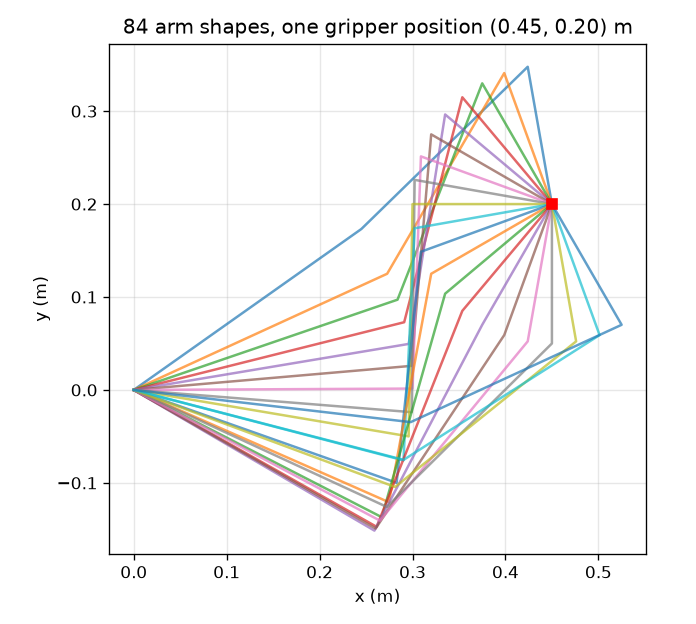
\includegraphics[width=0.85\linewidth]{figures/s02_redundancy_family.png}\\\small 84 arm shapes that all put the gripper on the same point (0.45, 0.20) m.\end{center}

\subsection*{E. Worked example}
Find the joint angles that put the gripper at (0.45, 0.20) m pointing along +x (phi = 0), for L = (0.30, 0.25, 0.15) m. Are they within +-120 degrees?
\begin{enumerate}[nosep]
\item Wrist: w = (0.45, 0.20) - 0.15 * (1, 0) = (0.30, 0.20) m, so \textbar{}w\textbar{}\textasciicircum{}2 = 0.13.
\item cos q2 = (0.13 - 0.0900 - 0.0625) / (2 * 0.30 * 0.25) = -0.0225 / 0.15 = -0.15, so q2 = +-98.63 degrees.
\item For q2 = +98.63: atan2(0.20, 0.30) = 33.69 degrees and atan2(0.25 * 0.9887, 0.30 + 0.25 * (-0.15)) = atan2(0.2472, 0.2625) = 43.28 degrees, so q1 = 33.69 - 43.28 = -9.59 degrees.
\item Then q3 = 0 - (-9.59) - 98.63 = -89.04 degrees. The other elbow choice gives (77.0, -98.6, 21.7) degrees in the same way.
\item All six angles have magnitude below 120 degrees, so both shapes are allowed. Check: both put the gripper at (0.45, 0.20) m with tool angle 0.
\end{enumerate}
\textbf{Answer.} Two arm shapes: (-9.6, 98.6, -89.0) degrees and (77.0, -98.6, 21.7) degrees; both within +-120 degrees.

\subsection*{F. Questions}
\begin{enumerate}[nosep]
\item \textbf{Conceptual.} A two-link arm with L1 = 0.30 m and L2 = 0.25 m has a hole of radius 0.05 m in its workspace. Why does adding a 0.15 m third link remove the hole, if the gripper's direction is free?
\item \textbf{Numerical.} Compute the reachable area of a two-link arm with L1 = 0.40 m and L2 = 0.20 m, and its smallest and largest radius.
\item \textbf{Graph and simulation interpretation.} From the graph of reachable fraction against joint limit, with L = (0.30, 0.25, 0.15) m, how much of the disk is lost at +-90 degrees, and what is the smallest 5 degree step of the limit that keeps 90 percent?
\item \textbf{Design and optimisation challenge.} Design: a work table 0.5 m x 0.3 m has its short edge 0.20 m in front of the base, centred on it. Choose L3 (keeping L1 = 0.30 m and L2 = 0.25 m) and the smallest joint limit in 5 degree steps so every point of the table is reachable. Justify it.
\end{enumerate}

\section{Session 3: Numerical inverse kinematics and a pick-and-place path}

\subsection*{A. Real-world problem}
A pick-and-place robot must follow a path: lift the part here, slide it there. The path is a list of gripper positions; the motors need joint angles for every one. For our 3-joint arm there is no single formula (one joint is spare), so the computer finds the angles by iteration, like Newton's method. What goes wrong when the arm is fully stretched, when the target is out of reach, or when a joint hits its limit? And how accurate is the result if a link is 1 mm longer than we think?

\subsection*{B. Concept and theory}
A small turn dq\_i of joint i moves the gripper by the i-th column of the Jacobian J, a 2 x 3 matrix, so a small change of all joints moves the gripper by J dq. If the gripper is off target by e, we want J dq = e. With three unknowns and two equations there are many answers; the pseudoinverse J\textasciicircum{}T (J J\textasciicircum{}T)\textasciicircum{}-1 e picks the smallest. Close to a singularity J J\textasciicircum{}T is nearly not invertible and the answer blows up, so we add a damping term: dq = J\textasciicircum{}T (J J\textasciicircum{}T + lambda\textasciicircum{}2 I)\textasciicircum{}-1 e (damped least squares). We repeat q = q + dq until e is tiny, capping the step at 0.1 rad per joint so a bad start cannot make the iteration jump. The singular values s1 \textgreater{}= s2 of J say how easily the gripper moves in its best and worst directions; the manipulability w = s1 s2 = sqrt(det(J J\textasciicircum{}T)) is zero when the arm is stretched, because J then has only one non-zero row. Because the arm has a spare joint, motion in the null space, dq = (I - J+ J) z, changes the shape of the arm and leaves the gripper where it is; we use it to push joints away from their limits. A straight-line path is timed with the quintic s(t) = 10 t\textasciicircum{}3 - 15 t\textasciicircum{}4 + 6 t\textasciicircum{}5, which starts and ends with zero speed and zero acceleration.

\begin{itemize}[nosep]
\item J: Jacobian: 2 x 3 matrix, metres of gripper motion per radian of each joint (m/rad)
\item e: position error, target minus current gripper position (m)
\item lambda: damping factor (m/rad)
\item s1, s2: singular values of J (m/rad)
\item w: manipulability s1 s2 (m\textasciicircum{}2/rad\textasciicircum{}2)
\item N: null-space projector I - J+ J (no unit)
\item s(t): path timing, 0 to 1 as t goes from 0 to 1 (no unit)
\end{itemize}

\begin{equation*}
J=\begin{pmatrix}-\sum_{k\ge1}L_k\sin c_k & -\sum_{k\ge2}L_k\sin c_k & -L_3\sin c_3\\ \ \ \sum_{k\ge1}L_k\cos c_k & \ \ \sum_{k\ge2}L_k\cos c_k & \ \ L_3\cos c_3\end{pmatrix},\qquad \Delta\mathbf p\approx J\,\Delta\mathbf q
\end{equation*}

\begin{equation*}
\Delta\mathbf q=J^{\mathsf T}\big(JJ^{\mathsf T}+\lambda^2I\big)^{-1}\mathbf e,\qquad \mathbf q\leftarrow\mathbf q+\Delta\mathbf q
\end{equation*}

\begin{equation*}
w=s_1s_2=\sqrt{\det\!\big(JJ^{\mathsf T}\big)}
\end{equation*}

\begin{equation*}
\Delta\mathbf q=J^{+}\mathbf e+\big(I-J^{+}J\big)\,k\,(\mathbf q_{\text{pref}}-\mathbf q),\qquad J^{+}=J^{\mathsf T}\big(JJ^{\mathsf T}+\lambda^2I\big)^{-1}
\end{equation*}

\begin{equation*}
s(t)=10t^3-15t^4+6t^5,\qquad \mathbf p(t)=\mathbf a+s(t)\,(\mathbf b-\mathbf a)
\end{equation*}

\begin{center}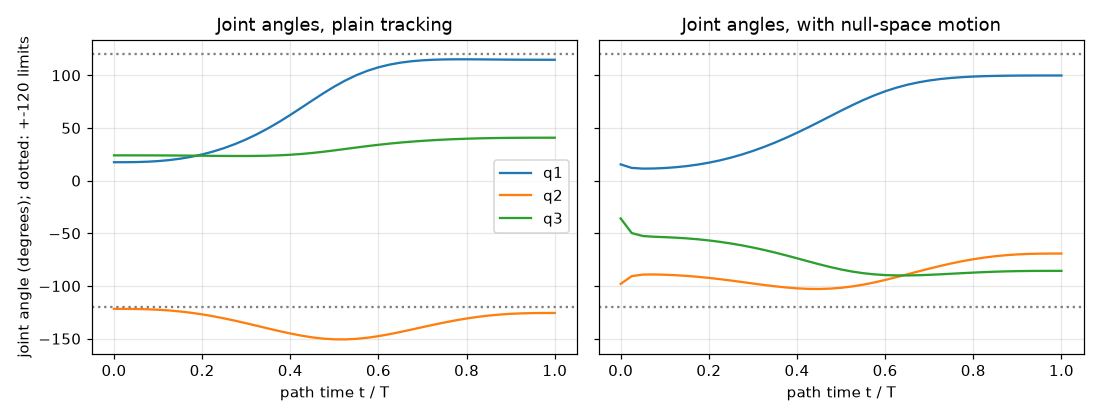
\includegraphics[width=0.85\linewidth]{figures/s03_path_joints.png}\\\small Joint angles along a 0.60 m straight path: plain tracking (left) and with null-space motion (right); dotted lines are the 120 degree limits.\end{center}

\subsection*{E. Worked example}
Reach the target (0.45, 0.20) m from the start q = (0.3, 0.3, 0.3) rad, lambda = 0.01. Trace the error, and compare the first step with the cap.
\begin{enumerate}[nosep]
\item Forward kinematics of the start: (0.586, 0.347) m, so the error is e = (-0.136, -0.147) m and \textbar{}e\textbar{} = 0.2006 m.
\item The raw damped step is dq = (-1.28, 1.56, 1.50) rad: far too large for a linear model, so it is scaled so that the largest joint change is 0.1 rad. The error becomes 0.1861 m.
\item Iterate: the error falls slowly at first while the steps are capped (0.168 m after 2 iterations, 0.091 m after 5), then very fast once the linear model is accurate.
\item After 8 iterations the error is 4.3e-4 m, after 9 it is 9.5e-7 m and after 10 it is 1.9e-9 m: each step squares the error, which is Newton-style convergence.
\item The iteration stops after 11 iterations with error below 1e-9 m, at q = (-21.0, 60.7, 59.0) degrees. Forward kinematics confirms the gripper is at (0.45, 0.20) m.
\end{enumerate}
\textbf{Answer.} The solver reaches (0.45, 0.20) m in 11 iterations; the error goes 0.2006, 0.1861, ..., 4.3e-4, 9.5e-7, 1.9e-9 m.

\subsection*{F. Questions}
\begin{enumerate}[nosep]
\item \textbf{Conceptual.} Why can a pure pseudoinverse demand enormous joint speeds near a fully stretched arm, and how does damping fix this? What does damping cost?
\item \textbf{Numerical.} Write the Jacobian of the stretched arm (all angles 0) with L = (0.30, 0.25, 0.15) m, and find its rank, its singular values and the manipulability.
\item \textbf{Graph and simulation interpretation.} In the log-log figure, what is the slope of the pseudoinverse line and what does it mean for the speed when the bend is ten times smaller? What does the damped line do?
\item \textbf{Design and optimisation challenge.} Design: plain tracking of the path from (0.25, -0.30) m to (0.25, 0.30) m (a start with q2 near -122 degrees) swings a joint to 150.7 degrees, but the motors stop at 120 degrees. Give two ways to fix it, with numbers, and one trade-off.
\end{enumerate}

\section{Real-world mini-project}
\textbf{Program a pick-and-place that avoids a no-go zone.} A part must move from the pick position (0.40, -0.20) m to the place position (0.40, 0.20) m on a table. A fixture, a disc of radius 0.06 m centred at (0.40, 0), sits exactly between them: the gripper must not enter it. The straight line between pick and place passes through its centre. Use \texttt{line\_path} and \texttt{track\_path} from Session 3 to route the gripper via one waypoint beside the zone, with quintic timing on each leg and joint limits of 120 degrees. Find the smallest sideways offset of the waypoint (in steps of 0.01 m) for which the gripper path keeps out of the zone. The zone applies to the gripper only; assume the links pass above the fixture.

\section{The path ahead}
\begin{enumerate}[nosep]
\item \textbf{Session 4: Whole-arm collision checking.} A checker that tests every link of the arm, not just the gripper, against the no-go zone, and a planner that picks the route and the elbow choice.
\item \textbf{Session 5: Speed limits and time-optimal timing.} A planner that stretches the move in time until no joint exceeds a speed limit.
\item \textbf{Session 6: Calibrate the link lengths.} A program that recovers the true link lengths from measured gripper positions at several poses.
\item \textbf{Session 7: A six-joint arm in 3D with orientation.} Forward and numerical inverse kinematics for a six-joint arm that sets position and orientation.
\item \textbf{Session 8: Animate the pick-and-place.} A looping animation of pick, carry, place and return, exported as a GIF, with the swept workspace and joint traces.
\end{enumerate}

\section{Answers and hints}

\subsection*{Session 1}
\begin{enumerate}[nosep]
\item \textbf{Conceptual.} Hint: Each joint angle is measured relative to the link before it. Solution: Joint 3 is measured relative to link 2, which itself points in the direction q1 + q2. So link 3 points at q1 + q2 + q3. If only joint 1 turns by 10 degrees, every link after it is carried along: the whole arm rotates rigidly by 10 degrees about the base, the tool angle increases by 10 degrees and the gripper moves round a circle centred on the base.
\item \textbf{Numerical.} Hint: The cumulative angles are 90, 0 and 0 degrees. Solution: Link 1 points up: (0, 0.30). Link 2 (cumulative angle 0) points along x: (0.25, 0). Link 3 (cumulative angle 0): (0.15, 0). Sum: (0.40, 0.30) m, exactly the block. Check: the distance from the base is sqrt(0.40\textasciicircum{}2 + 0.30\textasciicircum{}2) = 0.50 m, below 0.70 m, so it is reachable.
\item \textbf{Graph and simulation interpretation.} Hint: Set q1 = 0 to find the distance of the gripper from the base, then ask where that point lies on the circle. Solution: With q1 = 0 the gripper is at (0.632, 0.212) m, so its distance from the base is 0.667 m and that is the radius for every q1. The point is at angle atan2(0.212, 0.632) = 18.5 degrees from the x axis, so x is largest when q1 = -18.5 degrees, bringing it onto the x axis, where x = 0.667 m.
\item \textbf{Design and optimisation challenge.} Hint: Reach is limited by the total length; add the spare reach to the block distance. Solution: The arm must reach at least 0.50 + 0.10 = 0.60 m, which rules out 0.45 m. The smallest that qualifies is 0.60 m (0.70 and 0.85 also qualify). A longer arm reaches more but is heavier, needs bigger motors and, because a small joint error is multiplied by the distance, places the gripper less accurately. Assumption: the arm can be posed freely (no joint limits yet).
\end{enumerate}

\subsection*{Session 2}
\begin{enumerate}[nosep]
\item \textbf{Conceptual.} Hint: Where can the wrist be, and how far can the gripper be from the wrist? Solution: The wrist can be anywhere in the ring from 0.05 m to 0.55 m. The gripper is up to 0.15 m from the wrist in any direction (the direction is free). The hole has radius 0.05 m, which is smaller than 0.15 m, so every point of the hole is within 0.15 m of some wrist position in the ring. The hole disappears and the workspace is the full disk of radius 0.70 m. If the direction were fixed, the workspace would be the same ring shifted by 0.15 m, with the hole still there.
\item \textbf{Numerical.} Hint: Use area = 4 pi L1 L2 and the radii \textbar{}L1 - L2\textbar{} and L1 + L2. Solution: Smallest radius \textbar{}0.40 - 0.20\textbar{} = 0.20 m, largest 0.60 m. Area = 4 pi * 0.40 * 0.20 = 1.005 m\textasciicircum{}2. Check: pi (0.60\textasciicircum{}2 - 0.20\textasciicircum{}2) = pi * 0.32 = 1.005 m\textasciicircum{}2. A sanity check: the area must be smaller than the full disk pi * 0.60\textasciicircum{}2 = 1.131 m\textasciicircum{}2, and it is.
\item \textbf{Graph and simulation interpretation.} Hint: Read the curve at 90 and where it crosses the red line; the checkpoint prints the values. Solution: At +-90 degrees the reachable fraction is 0.613, so 0.387 of the disk is lost. The curve crosses 0.9 between 120 degrees (0.892) and 125 degrees (0.918), so the smallest 5 degree step is 125 degrees. The curve is steep at small limits and flattens near 180 degrees, so the last few degrees of motor range buy little.
\item \textbf{Design and optimisation challenge.} Hint: The farthest points are the far corners at (0.70, +-0.15) m; their distance must not exceed the total link length. Solution: The far corners are at sqrt(0.70\textasciicircum{}2 + 0.15\textasciicircum{}2) = 0.716 m, so the total length must be at least 0.716 m, i.e. L3 \textgreater{}= 0.166 m. With L3 = 0.15 m (total 0.70 m) only 0.956 of the table grid points are reachable; with L3 = 0.17 m (total 0.72 m) all of them are. The table is not close to the base (0.20 m), so the inner hole does not matter. Joint limits: with L3 = 0.17 m the table is fully reached at +-105 degrees but only 0.974 at +-100 and 0.839 at +-90, so choose +-105 degrees, and add margin (for example +-120) in practice. Trade-off: a longer last link gives a little more reach but adds weight at the end of the arm.
\end{enumerate}

\subsection*{Session 3}
\begin{enumerate}[nosep]
\item \textbf{Conceptual.} Hint: Think of the smallest singular value and the size of 1 / s2. Solution: At the stretched pose J has rank 1: the gripper cannot move along the arm at all. Just off it, the smallest singular value s2 is tiny, and the pseudoinverse divides by it, so a request to move along the arm gives joint speeds of about speed / s2 (6.4 rad/s for a 0.1 m/s request at a bend of 0.1 rad, 640 rad/s at 0.001 rad). Damping replaces 1/s2 by s2 / (s2\textasciicircum{}2 + lambda\textasciicircum{}2), which never exceeds 1 / (2 lambda). The cost: the gripper no longer follows the request exactly in the weak direction (it moves a little less than asked), and convergence is slower.
\item \textbf{Numerical.} Hint: With all angles 0 every sine is 0 and every cosine is 1; the columns are sums of lengths from joint i onwards. Solution: Row 1 (x) is -sum L\_k sin c\_k = 0 in all columns. Row 2 (y) is sum from i of L\_k cos c\_k = (0.70, 0.40, 0.15). So J = [[0, 0, 0], [0.70, 0.40, 0.15]], rank 1. The singular values are sqrt(0.70\textasciicircum{}2 + 0.40\textasciicircum{}2 + 0.15\textasciicircum{}2) = 0.82 m/rad and 0, so the manipulability is 0. Units: m/rad for J; the zero says the gripper cannot move along the arm.
\item \textbf{Graph and simulation interpretation.} Hint: Compare 6.4, 64 and 640 rad/s for bends of 0.1, 0.01, 0.001 rad. Solution: The line has slope -1: each time the bend is ten times smaller, the speed is ten times larger (6.4, 64, 640 rad/s). Speed is about 0.1 m/s divided by the smallest singular value, which is proportional to the bend. The damped line is nearly flat and tiny (0.57, 0.06, 0.01 rad/s for lambda = 0.05) because damping stops dividing by s2; it does not demand motion that the arm cannot make.
\item \textbf{Design and optimisation challenge.} Hint: One fix is to start from the other elbow choice; the other uses the spare joint with a null-space term. Solution: (1) Start from the other elbow choice (from the start q = (0.3, 0.3, 0.3) rad): plain tracking then keeps every joint below 99.5 degrees. (2) Keep the start, but add a null-space term k (q\_pref - q) with q\_pref = 0 and k = 0.1: the largest joint angle drops from 150.7 to 102.8 degrees with the same gripper path (error below 1e-6 m). Trade-off: the null-space motion moves the joints more per step (more joint speed) and shapes only joints that have slack; clipping alone cannot fix a path that the limits make impossible, so the target and path must be reachable within the limits to begin with.
\end{enumerate}

\section{How to join}
Read \texttt{CONTRIBUTING.md} in the repository, then pick an issue labelled \texttt{good first issue}. Repository: \url{https://github.com/KrunalPanchal1995/openrobotarm}

\end{document}
